\section{Theorems}

\newtheorem{theorem}{Theorem}[chapter]
\begin{theorem}
This is my first theorem.
\end{theorem}


\section{Axioms}
\newtheorem{axiom}{Axiom}[chapter]
\begin{axiom}
This is my first axiom.
\end{axiom}

\begin{axiom}
This is my second axiom in chapter 1.
\end{axiom}

\section{Tables}

This is my table. 

\renewcommand{\baselinestretch}{1}
\small\normalsize

\begin{table}[h]
\caption[Short title]{Overview of test cases used in this study.}
\begin{center}
\begin{tabular}{|c|c|c|c|}
\hline
Test & Quality & Setpoint & Manipulated \\
case & variable (QV) & for QV & variables (MVs)\\
\hline \hline
TE & G/H ratio & 1.226 & D-feed SP and Reactor Level SP\\
AZ & xB($H_2O$) & & Reflux flow and $5^{th}$ Tray temperature SP\\  
\hline
\end{tabular}
\end{center}
\label{test_over}
\end{table}

\renewcommand{\baselinestretch}{2}
\small\normalsize

My table is shown above.   Normally it is double-spaced but I have inserted a command (marked in blue) to make it single-spaced and then inserted a command (again in blue) to change the text back to double-spacing.

\

\subsection{Adding Extra Space between Text and Horizontal Lines}

\renewcommand{\baselinestretch}{1}
\small\normalsize

\setlength{\tablinesep}{5ex}

\begin{table}[h]
\caption{Table with Extra Space between the Text and Horizontal Lines.}
\begin{center}
\begin{tabular}{|p{.5in}|p{1in}|c|p{2.25in}|}
\hline
Test case& Quality variable QV)& Setpoint for QV & Manipulated  variables (MVs)\\
\hline \hline
TE & G/H ratio & 1.226 & D-feed SP and Reactor Level SP\\ \hline
AZ & xB($H_2O$) & & Reflux flow and $5^{th}$ Tray temperature SP \\
\hline
\end{tabular}
\end{center}
\label{test_over}
\end{table}

\renewcommand{\baselinestretch}{2}
\small\normalsize

The line \begin{verbatim}\usepackage{tabls}\end{verbatim} must be inserted in the preamble of your document.
The table is set up to be single-spaced by \begin{verbatim} \renewcommand{\baselinestretch}{1} \small\normalsize\end{verbatim} before \begin{verbatim}\begin{table}\end{verbatim}.  I set the first, second, and fourth columns as paragraphs, .5in, 1in, and 2.25in wide, respectively.  I then adjusted the separation between the words and the horizontal lines to 5ex by also adding \begin{verbatim}\setlength{\tablinesep}{5ex}\end{verbatim} before the \begin{verbatim}\begin{table}\end{verbatim} command.

After typing the table I change the document to be double-spaced from this point on.

\newpage


\section{Figures}

The figure on the following page is centered and the figure caption is indented and single-spaced.  Make sure you copy the last two lines \begin{verbatim}
\renewcommand{\baselinestretch}{2}\\
\small\normalsize\end{verbatim} to return to double-spacing of your text.

\begin{figure}
\begin{center}
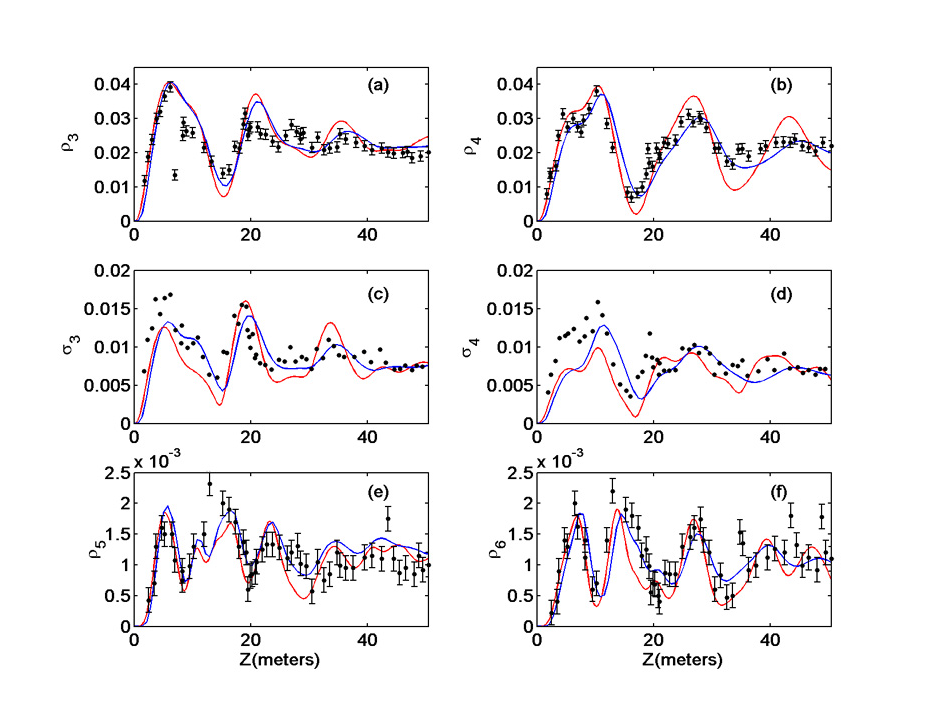
\includegraphics[width=6in]{nlsez55phaseornot.eps}
\end{center}
\renewcommand{\baselinestretch}{1}
\small\normalsize
\begin{quote}
\caption[Figure with caption indented]{This figure caption is indented and single-spaced.  Comparison between the experimental measurements \cite{hart1} (black), the random initial condition NLSE model excluding phase noise (dashed curves) and the stochastic phase noise NLSE model (solid curves) showing the first- and second-order sideband evolution as a function of fiber length for P$_{0} = 5.5$\,W, $\Omega = 366$\,GHz, $\Delta\nu = 0.5$\,GHz, $\gamma = 0.019$\,W$^{-1}$m$^{-1}$, and $\beta^{(2)} = 55$\,ps$^2$/km: dynamical evolution of the: (a) power in the first-order blue-shifted sideband, (b) power in the first-order red-shifted sideband, (c) fluctuations in the first-order blue-shifted sideband, (d) fluctuations in the first-order red-shifted sideband, (e) power in the second-order blue-shifted sideband, (f) power in the second-order red-shifted sideband. \label{fig:fig27}}
\end{quote}
\end{figure} 
\renewcommand{\baselinestretch}{2}
\small\normalsize

The first figure is Fig.\ref{fig:fig27}.   Please note that the figure label should be placed inside the figure caption.  
\newpage

The next figure is placed landscape.  It is Fig.~\ref{fig:mpc}.

\begin{landscape}
\renewcommand{\baselinestretch}{1}
\small\normalsize
\begin{quote}
\begin{figure}
\begin{center}
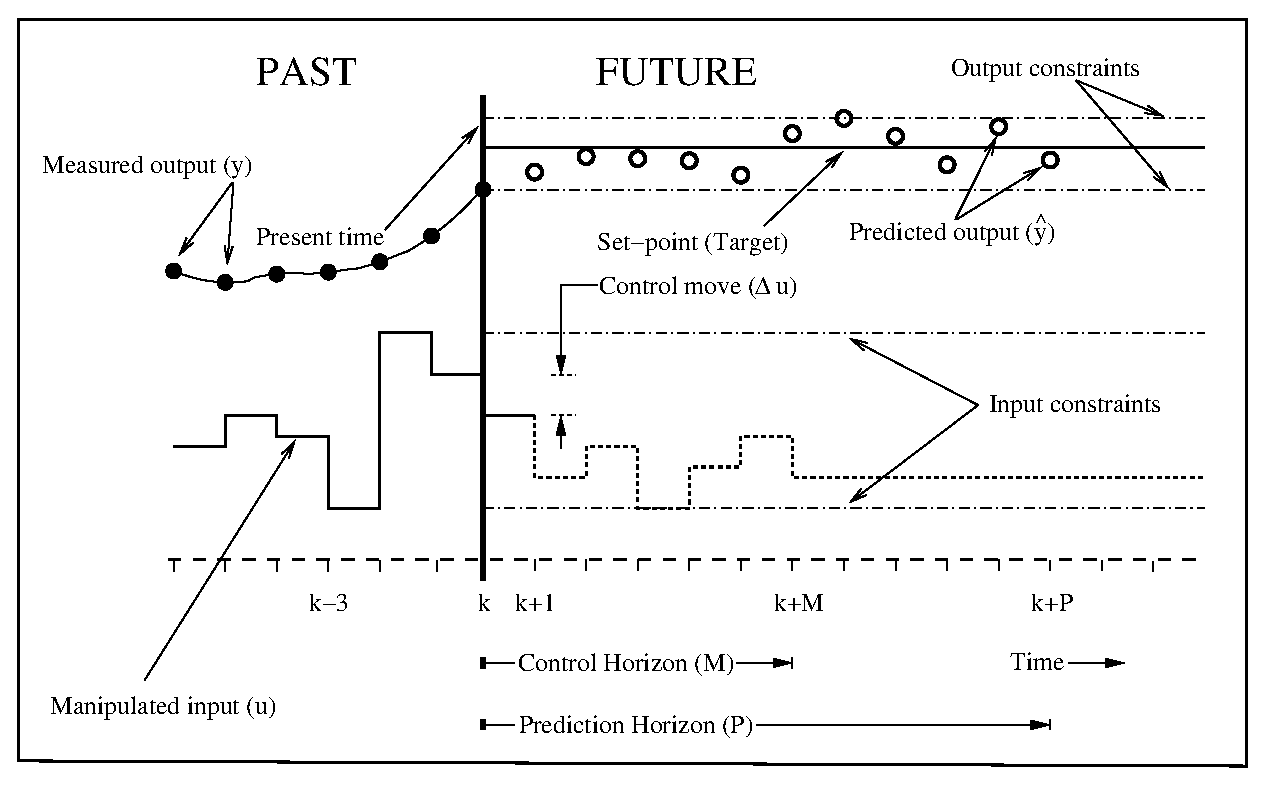
\includegraphics[width=8.2in]{mpc.eps}
\end{center}
\caption{Schematic illustrating receding horizon control.
\label{fig:mpc} }
\end{figure}
\end{quote}
\renewcommand{\baselinestretch}{2}
\small\normalsize
\end{landscape}

This is a my second figure which was placed landscape.  Although I have used the same figure, I have renamed the label to fig:mpc-1.  The second figure now becomes Figure~\ref{fig:mpc-1}.
\begin{landscape}
\renewcommand{\baselinestretch}{1}
\small\normalsize
\begin{quote}
\begin{figure}
\begin{center}
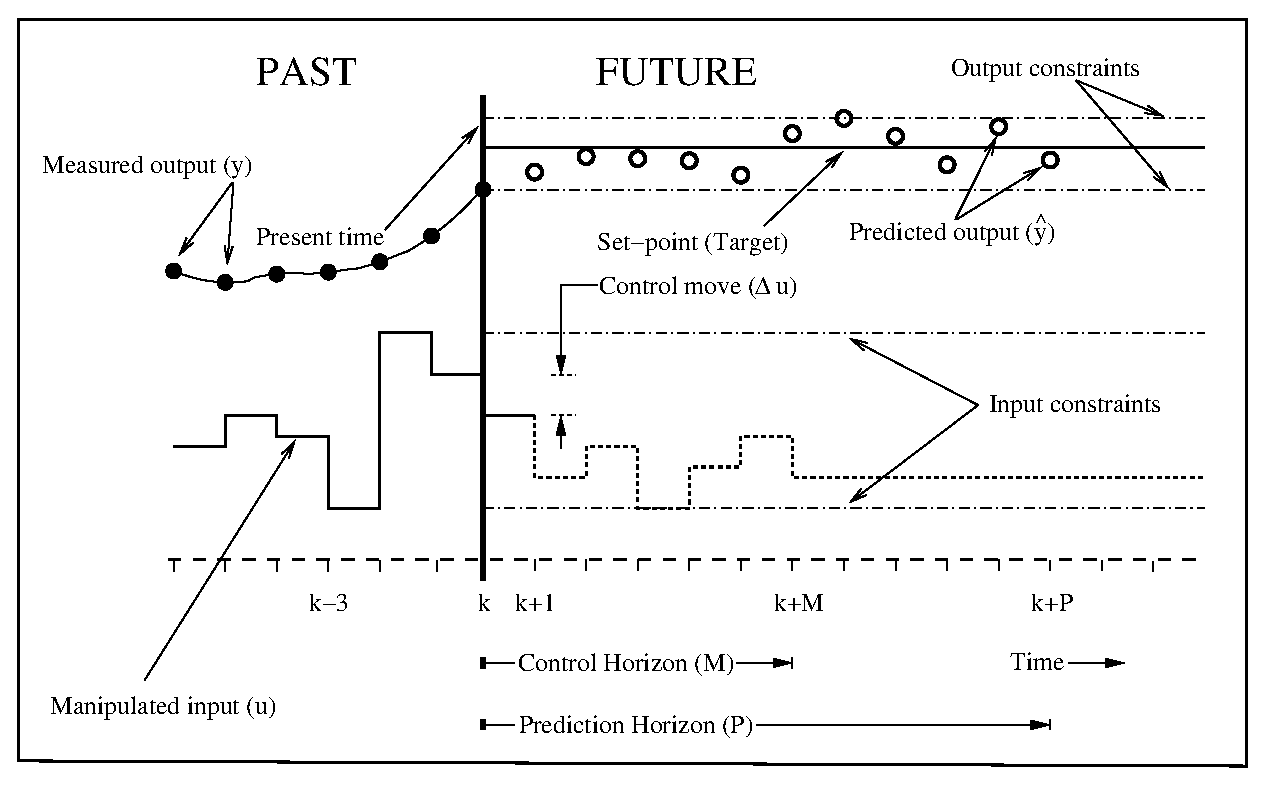
\includegraphics[width=8.2in]{mpc.eps}
\end{center}
\caption[Figure placed landscape on page]{Schematic illustrating receding horizon control. \label{fig:mpc-1}}
\end{figure}
\end{quote}
\renewcommand{\baselinestretch}{2}
\small\normalsize
\end{landscape}

\subsection{Numbering Figures}

If you wish your figures to be numbered 1-100 without any reference to the chapter (e.g., Figure 1.1, 2.1, etc.), change the first line of your mainthesis.tex file to read \begin{verbatim}"\documentclass[12pt]{thesis-2}".\end{verbatim}  

\subsubsection{This is a Subsubsection}

This is my first subsubsection in Chapter 1.


\section[Short Titles]{Short Titles in the Table of Contents, List of Figures, or List of Tables}

The Table of Contents, List of Figures, or List of Tables usually show the entire title of a section, subsection, etc. or table, or the entire caption of a figure.  If you put a short title in square brackets after \begin{verbatim} \section, \table, or \figure, \end{verbatim} the short title will show in your Table of Contents or lists.

\renewcommand{\baselinestretch}{1}
\small\normalsize

\begin{verbatim}
\section[Short Title]{Title of Section} 
\subsection[Short Title]{Title of Subsection} 
\end{verbatim}

or when using a caption in a figure or table
\begin{verbatim}
\caption[Short Caption]{Full text of the caption.}
\end{verbatim}

\renewcommand{\baselinestretch}{2}
\small\normalsize


\section{Figures on Text Page}

Normally figures in the thesis are placed on a page by themselves.  The following figure is placed on the page with text before and after the figure by adding [!!h] after \begin{verbatim} \begin{figure}[!!h] \end{verbatim}.  Please note that the figure label is placed within the caption.

\renewcommand{\baselinestretch}{1}
\large\normalsize

\begin{verbatim}
\begin{figure}[!!h]
 \begin{center}
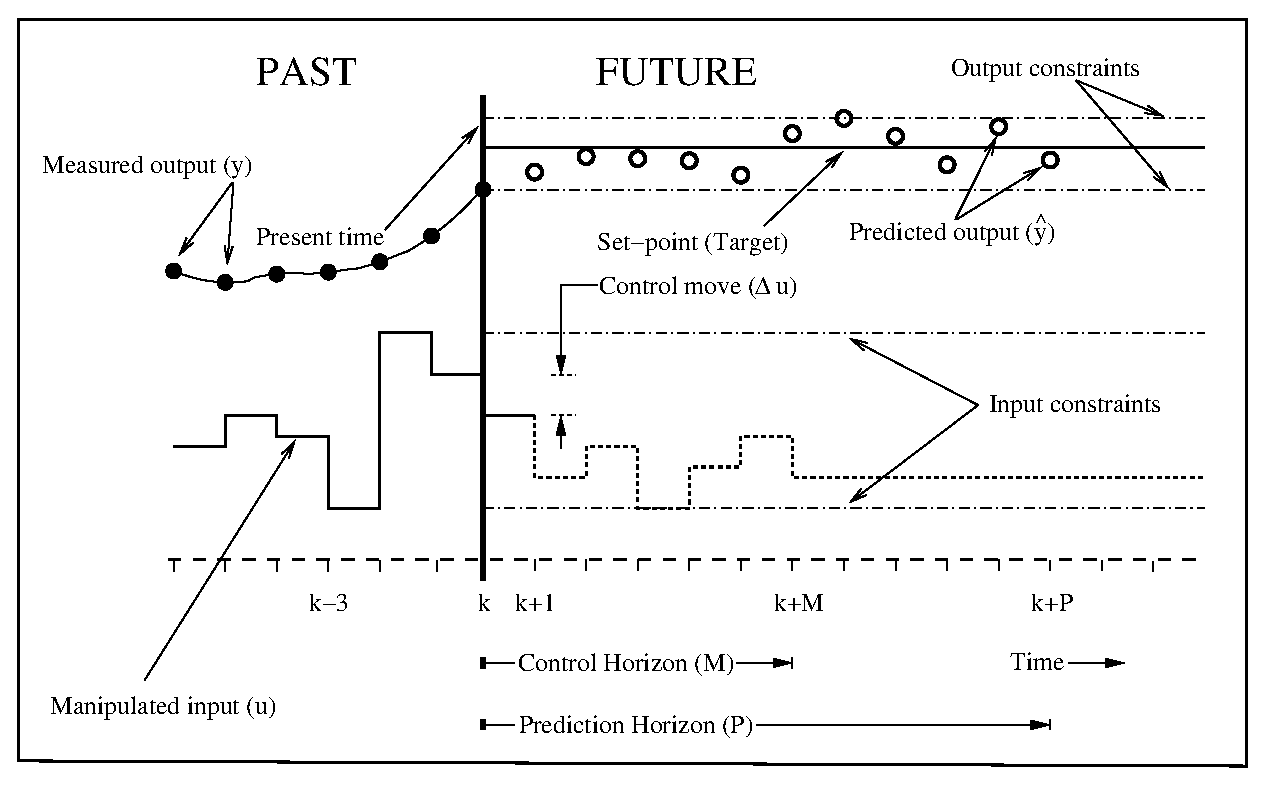
\includegraphics[width=5in]{mpc.eps}
\end{center}
\caption[Short title]{Schematic illustrating receding horizon control.
\label{fig:mpc-2}}
\end{figure}
\end{verbatim}

\begin{figure}[!!h]
 \begin{center}
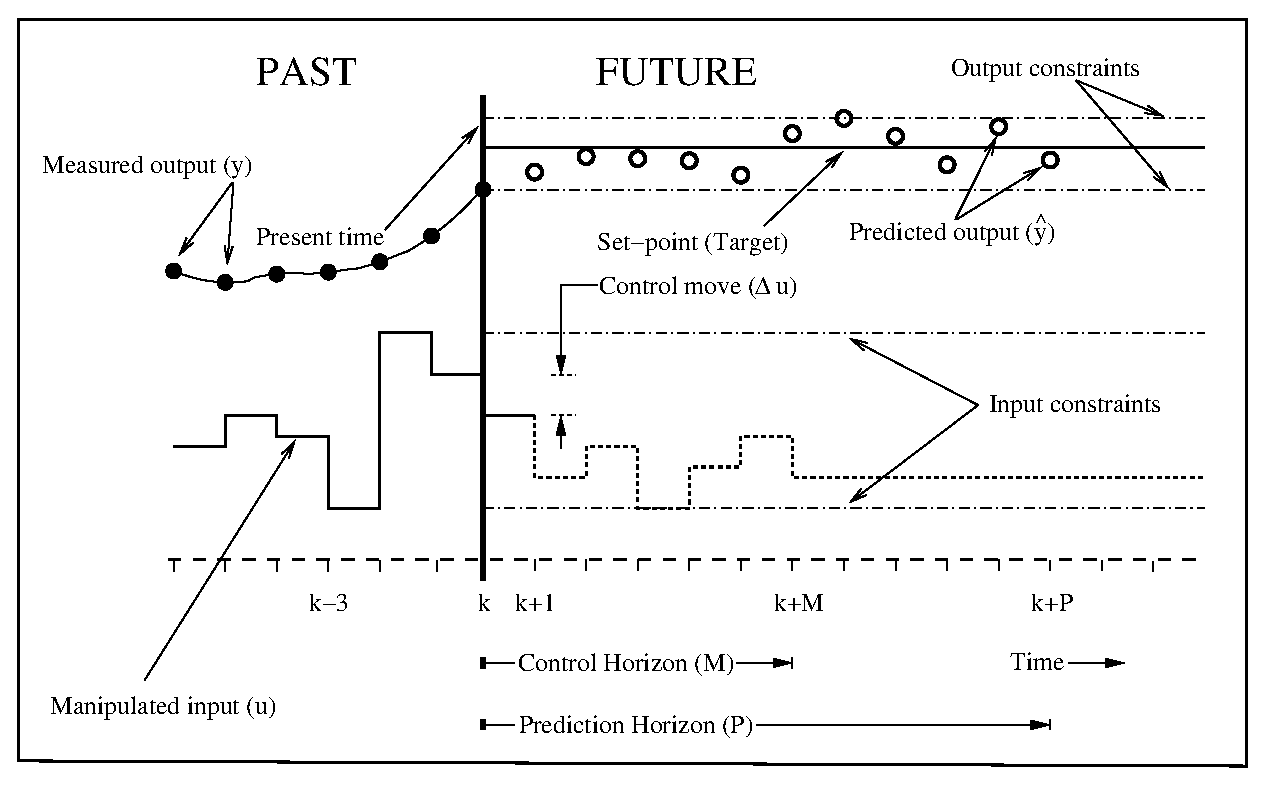
\includegraphics[width=5in]{mpc.eps}
\end{center}
\caption{Schematic illustrating receding horizon control. \label{fig:mpc-2}}
\end{figure}

\renewcommand{\baselinestretch}{2}
\large\normalsize

This does not necessarily mean that the text before and after the figure will be exactly what you want.  Remember Latex will place the figure where it will fit on the page the best.   The previous figure is Figs.~\ref{fig:mpc-2}. 

\section{Wrapping Text around Figure}


\renewcommand{\baselinestretch}{1}
\begin{wrapfigure}{r}{0.4\textwidth}
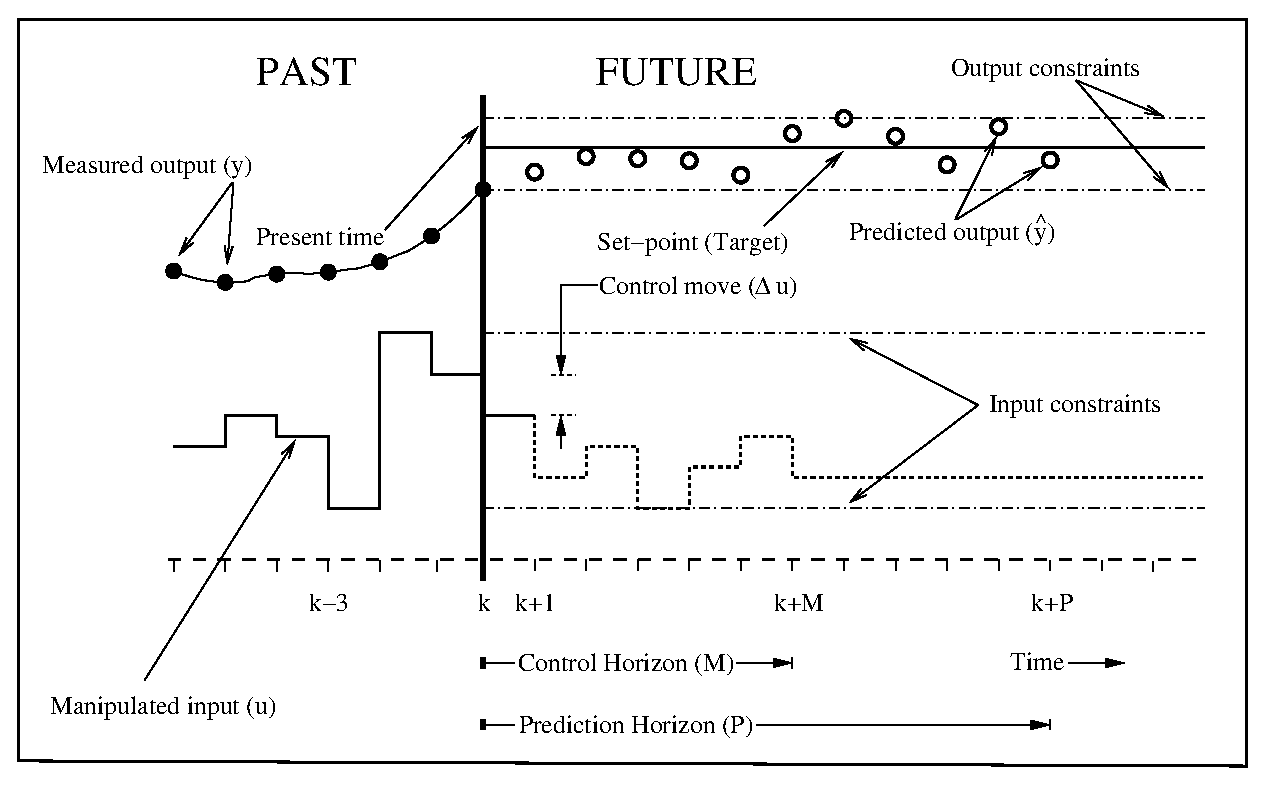
\includegraphics[width=0.4\textwidth]{mpc.eps}
\caption{ Text wrap around figure. \label{fig:test}}
\end{wrapfigure}

\renewcommand{\baselinestretch}{2}
\large\normalsize

By way of summary, at the end of the activity, I reminded the class of what we'd done:  by considering relatively nearby galaxies whose distance we had measured by some other means, we were able to establish a relationship locally between redshift and distance.  
By way of summary, at the end of the activity, I reminded the class of what we'd done:  by considering relatively nearby galaxies whose distance we had measured by some other means, we were able to establish a relationship locally between redshift and distance.  
By way of summary, at the end of the activity, I reminded the class of what we'd done:  by considering relatively nearby galaxies whose distance we had measured by some other means, we were able to establish a relationship locally between redshift and distance.  
By way of summary, at the end of the activity, I reminded the class of what we'd done:  by considering relatively nearby galaxies whose distance we had measured by some other means, we were able to establish a relationship locally between redshift and distance.  See Fig.~\ref{fig:test}.


\section{LaTeX -- A Typesetting Program}

A 13-page explanation of some of the features of LaTeX can be downloaded from http://www.jgsee.kmutt.ac.th/exell/General/LaTeX.html.


\section{Using Bibtex}

Using Bibtex with Latex documents is not difficult.  The bulk of the work is organizing your bibtex file, which is a data base compiled by you of the articles, books, etc. which you use in the bibliographies or reference sections of your publications.  

I have linked several files to this webpage, which will be helpful when you are using Bibtex.  These files can be downloaded from \newline
http://www.ireap.umd.edu/ireap/theses/bibtex.  Please read the file "BibtexInstructions.pdf".  The first two pages explain how to set up and run Bibtex; the remaining pages were taken from a published article and show how the references were cited in the .tex file.   The files BibtexInstructions.tex, Galactic.bib, Dottie.bib are the original .tex files used for BibtexInstructions.pdf.  The file BibtexSamples.tex contains examples of the information needed for the various publications you wish to reference (e.g., articles in refereed journals, books, unpublished articles, conference proceedings, etc.).

If you have questions concerning Bibtex, please contact me at 301-405-4955 or dbrosius at umd.edu.

\section{Using Natbib}

Another option of citing references in the bibliography is using Natbib instead of Bibtex.  You must still create a bibtex file, as noted above.  The command "backslash cite" cannot be used with natbib; instead "backslash citet" and "backslash citep" must be used.    "backslash citet" is used to show reference in the text (e.g., Eq.\ 8 in Reiser,1996 shows ...); "backslash citep" is used in the parenthetical (e.g., Eq.\ 8 (Reiser, 1996) shows ...).  

\begin{verbatim}
Add in preamble -- \usepackage[option]{natbib} 

Add at bottom of mainthesis.tex file --
\bibliography{name of your bibtex file}
\bibliographystyle{plainnat, abbrnat, or unsrtnat}
\end{verbatim}

Typesetting:   Latex, Bibtex, Latex, Latex

The reference sheet for natbib usage can be found at \newline "http://merkel.zoneo.net/Latex/natbib.php".

\section{APS Physical Review Style and Notation Guide}

The following style guide may be downloaded from The American Physical Society at http://forms.aps.org/author/styleguide.pdf:  Physical Review Style and Notation Guide, published by The American Physical Society, compiled and edited by Anne Waldron, Peggy Judd, and Valerie Miller, February 1993.  It may be old, but it is very useful.
